\subsubsection{Gestão de grupos de trabalho}

Um aluno, para submeter uma entrega, precisa de pertencer um grupo de trabalho que verifique as restrições impostas pelo docente.

É nesta página que um aluno, pode consultar os grupos de trabalho do projeto, criar o seu novo grupo ou adicionar elementos ao seu grupo atual.\\

Nesta página foram tomadas várias decisões, de forma a melhorar o funcionamento do sistema e a segurança dos utilizadores relativamente a grupos e entregas.

\begin{itemize}
  \item \textbf{Todos os elementos do grupo podem adicionar novos elementos}

    Esta decisão foi tomada com o objetivo de dar flexibilidade à criação de grupos de trabalho. Como as entregas podem depender do grupo de trabalho, optou-se por não dar a responsabilidade de adição de elementos apenas a um utilizador.

  \item \textbf{Um aluno pode abandonar um grupo, mas não pode remover outros elementos}

    Com esta decisão pretende-se garantir a segurança a um aluno, assegura-se assim que um elemento não seja removido de um grupo sem a sua aprovação, o que poderia resultar em entregas não submetidas e consequentemente não ser avaliado.

  \item \textbf{Um aluno só pode abandonar um grupo, se esse grupo ainda não tiver efetuado entregas}

    Depois da submissão de uma entrega, o grupo não pode perder elementos, se assim fosse, o processo de avaliação tornar-se-ia mais complexo e difícil de automatizar. Poderiam surgir também problemas de segurança para os restantes elementos do grupo, uma vez que haveriam entregas partilhadas.

  \item \textbf{Só podem ser adicionados elementos que ainda não tenham grupo de trabalho no projeto}

    Garante-se assim que um utilizador só num grupo de trabalho, com esta decisão pretende-se resolver ambiguidades no momento de submissão uma entrega.

  \item \textbf{So podem ser adicionados novos elementos, se o grupo ainda não tiver o número máximo de elementos imposto pelo docente}

    Um grupo com mais elementos que o permitido não conseguiria efetuar submissões de entregas, ao colocar esta restrição, garante-se assim que nenhum aluno adiciona todos os elementos de uma unidade curricular, o que poderia dificultar o normal funcionamento do sistema.

  \item \textbf{Se um aluno não pertence a nenhum grupo de trabalho, pode criar um novo grupo}

    Se um aluno ainda não tiver um grupo de trabalho, pode criar e adicionar elementos ao seu novo grupo de trabalho, até que as restrições impostas pelo docente sejam realizadas.

\end{itemize}

É importante referir que um aluno pode consultar os grupos que ainda se encontram incompletos, e pode adicionar mais que um elemento em simultâneo no seu grupo de trabalho.\\

Na Figura~\ref{fig:student_groups_add} pode ser consultada uma imagem demonstrativa da página desenvolvida, para o caso de um aluno já pertencer a um grupo de trabalho.

\begin{figure}[H]
  \centering
  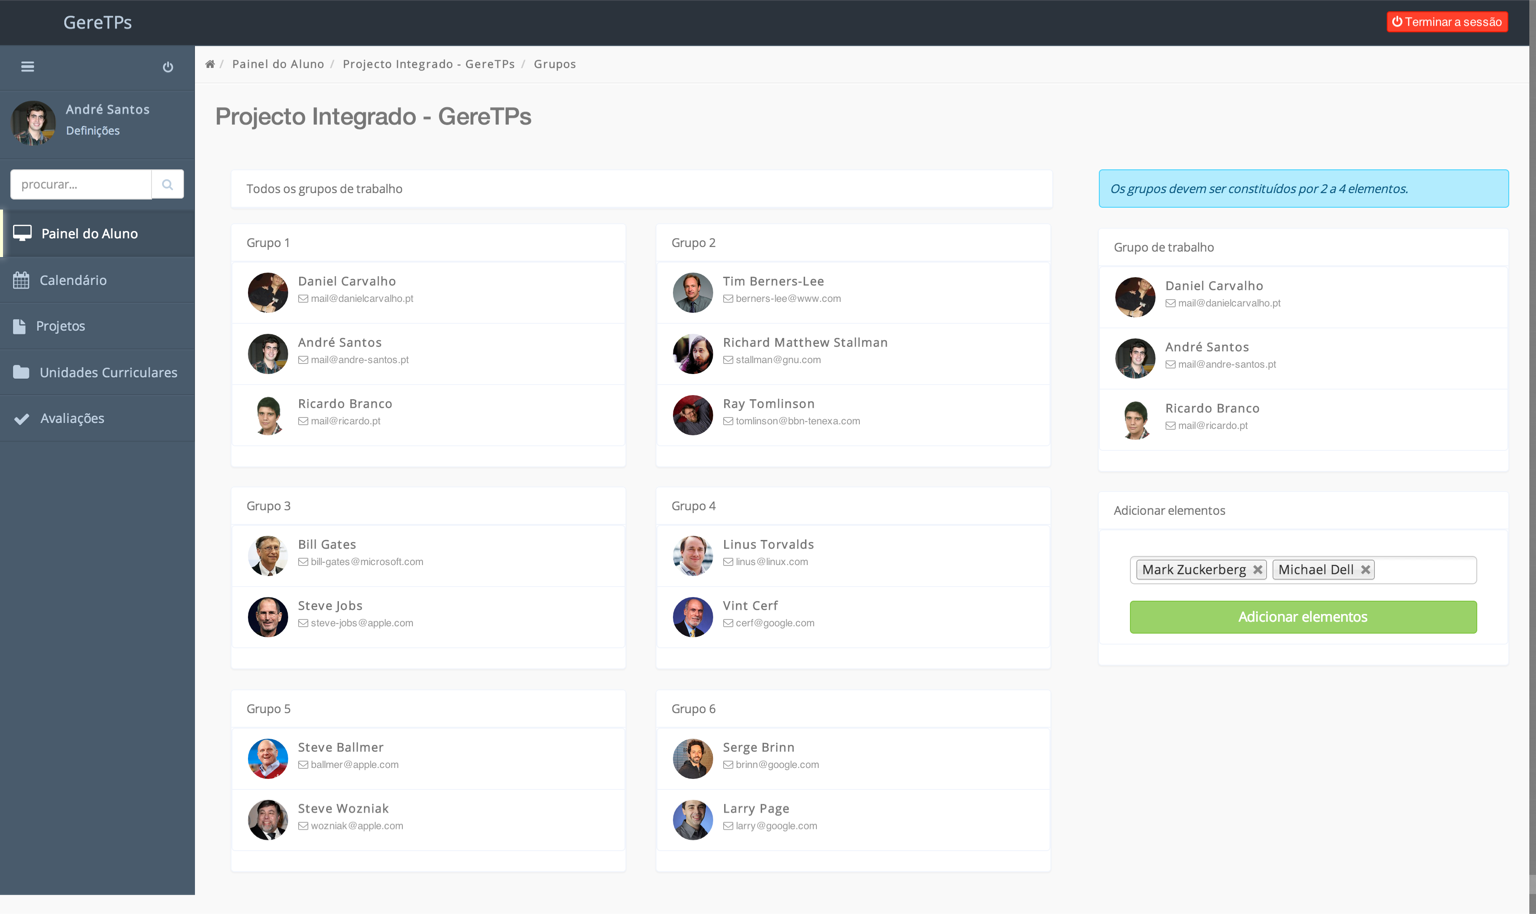
\includegraphics[width=1\textwidth,center]{images/implementacao/alunos/groups_add}
  \caption{Página de gestão de grupos de trabalho}
  \label{fig:student_groups_add}
\end{figure}

E na Figura~\ref{fig:student_groups_add} pode ser consultada uma imagem demonstrativa da página desenvolvida, para o caso de um aluno ainda não pertencer a nenhum grupo.


\begin{figure}[H]
  \centering
  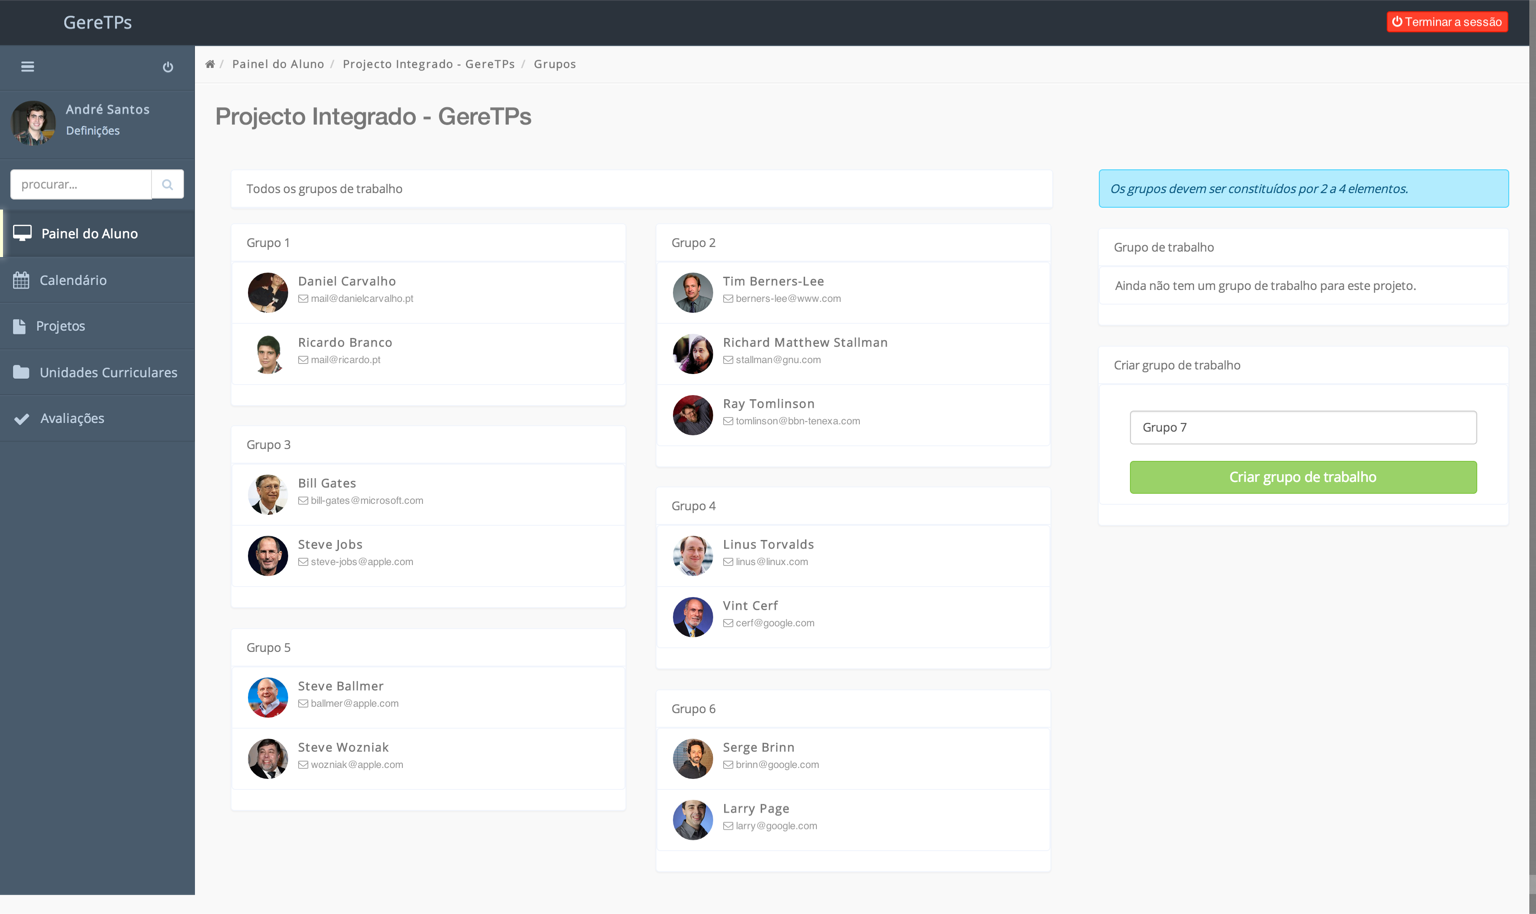
\includegraphics[width=1\textwidth,center]{images/implementacao/alunos/groups_create}
  \caption{Página de gestão de grupos de trabalho}
  \label{fig:student_groups_create}
\end{figure}
